\chapter{Contexto}


\section{Recuperación de información}
La \textbf{\acrfull{RI}} es una disciplina que trata de modelar, diseñar e implementar sistemas capaces de promocionar acceso basado en contenidos. \cite{RIspaBook}

En general un sistema de \acrshort{RI} recibe una petición o consulta  del usuario y debe devolver de entre su conjunto de información las unidades relacionadas con la consulta. 

Estas unidades pueden representar cualquier tipo de elemento: ficheros de texto, imágenes, archivos de audio, etc. De forma genérica se denominan \textbf{documentos} así como al conjunto de información se le denomina \textbf{colección}.



\subsection{Relevancia y similitud}
La \textbf{relevancia} hace referencia a la relación entre la consulta de un usuario y los documentos recuperados. Por ello intuitivamente se entiende que un documento es relevante para una consulta concreta si contribuye a satisfacer la necesidad de información expresada por la misma. Aunque el concepto pueda parecer claro, la relevancia no es para nada absoluta, es una media subjetiva que depende de varios factores como quien la valore o como se haya planteado la consulta inicial.

Respecto a la \textbf{similitud} esta es una medida de semejanza entre documentos o entre documentos y consultas. Otra vez más nos encontramos ante una medida relativa y que se puede medir de diversas maneras: comparación de cadenas de texto, uso de un mismo vocabulario, que dos documentos pertenezcan al mismo autor, que dos documentos tengan múltiples referencias comunes...\cite{ApuntesRI}


\subsection{Las tres dimensiones de la \acrshort{RI}}
Se puede decir que las tres dimensiones principales de la \acrshort{RI} son:\cite{RIspaBook}

\subsubsection{Acceso a la información}
Como puede acceder un usuario a los datos. Existen diversos paradigmas de búsqueda:
\begin{itemize}
	\item \textbf{Clasificación}: cada documento pertenece a clases y estas se pueden usar como jerarquías.
	\item \textbf{Agrupamiento}: documentos se agrupan en conjuntos.
	\item \textbf{Filtrado}: se selecciona un subconjunto de documentos.
	\item \textbf{Recomendación}: los documentos se presentan al usuario basados en su interacción previa con el sistema.
	\item \textbf{Resumen}: fragmentos de documentos utilizados para reducir la información presentada al usuario, muy típico de motores de búsqueda web.
\end{itemize}
\subsubsection{Tipos de información}
Hoy en día vivimos en una marea de información muy heterogénea y creciente lo que hace complicado definir los distintos tipos, por citar los principales actualmente:
\begin{itemize}
	\item \textbf{Documentos textuales} como paginas web o \acrshort{PDF}.
	\item \textbf{Partes de un documento}, capítulos o secciones de este.
	\item \textbf{Búsqueda de información multimedia}: como canciones o vídeos a partir de propiedades perceptibles o incluso de otros elementos multimedia, la búsqueda de imágenes en Google imágenes por ejemplo.
	\item \textbf{Búsqueda de e-mails}: implementado en cualquier cliente de correo web o nativo.
	\item \textbf{Búsqueda geográfica}: por nombre del lugar, sitios cercanos...
\end{itemize}
\subsubsection{Colección}
Guarda relación con los documentos que pueden ser buscados y se pueden clasificar tres tipos en función del tamaño:
\begin{itemize}
	\item \textbf{Personal}: ficheros del dispositivo del usuario.
	\item \textbf{Corporativa}: documentos de una empresa, algo más compleja, supone búsqueda en múltiples ubicaciones conectadas en red.
	\item \textbf{Web}: cualquier documento web, el volumen de datos y la infraestructura es descomunal.
\end{itemize}


\subsection{Componentes de un sistema de \acrshort{RI}}
De manera general un sistema de \acrshort{RI} se compone de los elementos que se observan en la siguiente figura. Ha de contar una interfaz de usuario encargada de recoger las peticiones y mostrar los resultados. Sera necesario interpretar estas consultas para convertirlas en términos que el sistema pueda entender.

\begin{figure}[h]
	\centering
	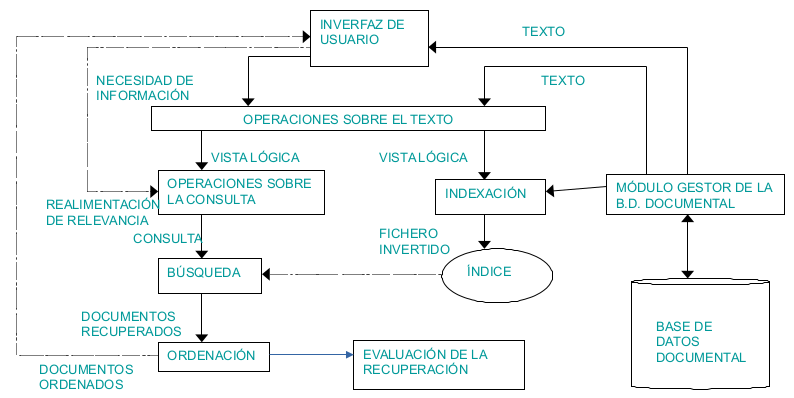
\includegraphics[width=\linewidth]{imagenes/componentes_ri}
	\caption{Componentes de un sistema RI \cite{ApuntesRI}}
	\label{fig:componentes RI}
\end{figure}

Una vez hecho esto el algoritmo de búsqueda encontrara los documentos que sean relevantes para la consulta, tras esto sera necesario puntuar estos documentos recuperados y devolver esta lista puntuada al usuario.

Para realizar este proceso de búsqueda y priorización se servirá del \textbf{índice}, una o varias estructuras de datos que permiten optimizar la búsqueda sobre una colección. En su forma más básica se trata de una estructura que relaciona términos con los documentos en los que aparecen, de modo que si una consulta contiene esos términos se devuelven los documentos que los contienen.

\subsection{Modelos}
\label{subsc:modelos}
Se puede definir un modelo de \acrshort{RI} como una especificación de la forma de representar documentos, consultas y realizar comparaciones entre ambos \cite{ApuntesRI}. El objetivo final es calcular una puntuación para cada documento dada una consulta especifica que determine el grado de relevancia de este, utilizando esa medida se puede llevar a cabo una ordenación o ranking de los documentos. 

Los modelos clásicos a pesar de ser los más básicos sirven como base para crear otros más complejos como alguno de los que se hablará posteriormente. Estos modelos clásicos son:\cite{RIspaBook}

\begin{list}{}{}
	\item  El \textbf{Modelo booleano} basado en teoría de conjuntos y lógica booleana. Se define el conjunto \textit{V} como todas las palabras clave de la colección, \textit{V = \{\(t_1, t_2, ..., t_M\)\}}, así mismo se define el conjunto \textit{D} como el conjunto de todos los documentos de la colección \textit{D = \{\(d_1, d_2, ..., d_n\)\}}. 
	
	Cada documento \(d_i\) se representa por tanto como un conjunto de términos que aparecen en él, este es un subconjunto de \textit{V}. Las consultas en este modelo se representan mediante las operaciones booleanas típicas AND, OR y NOT.
	
	\item El \textbf{Modelo vectorial} modela los documentos y consultas como vectores de términos en un espacio vectorial de dimensión definida por el número de términos de la colección. 
	
	Cada documento es por tanto un vector en dicho espacio vectorial. Usando los conjuntos descritos en el modelo previo se puede definir un documento \(d_i\) como el vector de términos \(\vec{d_i} = (w_{1,i}, w_{2,i}, ..., w_{M,i})\) donde \(w_{i,j}\) representa el peso del término i en el documento j.
	
	Queda por determinar el esquema de pesos y la función de similitud entre vectores.
	
	\item El \textbf{Modelo probabilístico} pretende expresar la relevancia de los documentos utilizando la teoría de probabilidades, por tanto se define \(P(Rel|d, q)\) como la probabilidad de que dado un documento \textit{d} y una consulta \textit{q} el documento sea relevante con cierta probabilidad. 
	
	Simplificando la notación a $P(Rel|d)$ y usando el \gls{Bayes}\glsrefentry{Bayes} podemos transformar el cálculo de esa probabilidad en:
	\begin{equation}
	P(Rel|d) = \frac{P(d|Rel)P(Rel)}{P(d)}
	\end{equation}
	
	
	La función de similitud en el modelo probabilístico se expresa como:
	\begin{equation}
	sim(q,d) = \frac{P(Rel|d)}{P(\overline{Rel}|d)}
	\end{equation}
	Es decir el ratio entre la probabilidad de que un documento sea relevante y no para \textit{q}. 
	
	Aplicando la transformación anterior esta función queda como:
	\begin{equation}
	sim(q,d) = \frac{P(d|Rel)}{P(d|\overline{Rel})}\frac{P(Rel)}{P(\overline{Rel})} \approx \frac{P(d|Rel)}{P(d|\overline{Rel})}
	\end{equation}
	Donde $\frac{P(Rel)}{P(\overline{Rel})}$ se conoce como característica independiente de consulta\label{modelProb} al suponer la relación entre las probabilidades de escoger un documento al azar y que este sea relevante o irrelevante, se suele eliminar como simplificación. 
	
	Por otro lado $\frac{P(d|Rel)}{P(d|\overline{Rel})}$ supone la relación entre la probabilidad sabiendo que un documento es relevante este sea \textit{d} y su inversa. Estas probabilidades resultan más fáciles de calcular y son las utilizadas en estos modelos.
	
	
\end{list}
\subsection{Contexto histórico}
La historia de la \acrshort{RI} comienza antes de la era digital. Como ejemplo las tablas de contenidos e índices de un libro forman un sistema de \acrshort{RI} a pequeña escala, los índices relacionan \gls{termIndex} con su ubicación en el documento de forma similar a un glosario de términos, ver \glsrefentry{termIndex} .

Esto es lo que se conoce como búsqueda \textbf{pre-coordinada} donde los términos de búsqueda o consultas están definidas de antemano, esto hace que se pueda organizar muy bien la información (como se hace en una biblioteca por ejemplo), pero requiere que el usuario conozca estos términos y no supone un método muy escalable teniendo en cuenta el volumen de información manejado en sistemas actuales. Por ello surgió la \textbf{post-coordinación} en la década de 1950 que se basa en definir las consultas en el momento de la búsqueda, dándole libertad al usuario.

A este último enfoque pertenecen la mayoría de los sistemas actuales, los cuales recibieron un enorme impulso con el desarrollo de la web iniciado en 1989 por Tim Berners-Lee en el CERN. Los primeros buscadores web de la forma que los conocemos hoy surgieron entorno a 1994, sistemas como Lycos o Altavista. 

La búsqueda de documentos en la web siempre ha resultado un reto debido a su naturaleza heterogénea, la propuesta de unos jóvenes estudiantes de la universidad de Stanford en 1998 supuso una revolución y asentó lo que hoy conocemos como buscador. Esa propuesta fue el algoritmo \textit{PageRank}\cite{PageRankPaper} y esos chicos eran Larry Page, Sergey Brin, Rajeev Motwani y Terry Winograd; los dos primeros fundaron poco después una empresa llamada Google, que a día de hoy es el buscador más utilizado. \cite{searchEngineShare}

Hoy en día existe una dependencia casi absoluta por los motores de búsqueda para navegar por internet, lo que hace de este un tema tan crucial en el que aún se sigue trabajando, con retos aún por delante como el enorme tamaño que ha alcanzado la web, la heterogeneidad de contenido con cada vez más contenidos multimedia o el acceso desde cualquier tipo de dispositivo y desde cualquier lugar. 

\section{Bibliometría}
\label{sc:bibliometria}
\subsection{Definición}
La \textbf{bibliometría} se puede definir como el análisis estadístico de publicaciones escritas. Sus métodos se suelen utilizar para ofrecer un análisis cuantitativo de la literatura académica \cite{de2009bibliometrics}. Se relaciona mucho con la \textbf{cienciometría} que se puede entender como el estudio cuantitativo de la ciencia de forma general \cite{DBLP:journals/corr/abs-1208-4566}. 

Específicamente para este trabajo resulta destacable el enfoque de poder medir la importancia de trabajos científicos de forma cuantitativa y como esto se puede utilizar para mejorar los resultados de un sistema \acrshort{RI}. Yendo al uso más particular que se llevara a cabo durante el desarrollo de este trabajo ambas disciplinas proponen una serie de medidas particulares, algunas de las cuales comentaré en el siguiente apartado.

\subsection{Medidas}
\subsubsection{Número de citas} \label{numero_citas}
Esta es una de las métricas más directas y sencillas, se basa la premisa de que un documento científico es más relevante si cuenta con mayor número de citas. Actualmente se encuentra disponible en casi cualquier plataforma bibliográfica como Google Schoolar, Scopus o Web of Science. 

Sobre esta métrica básica se han construido muchas posteriormente como el impacto de citas (media de citas por documento), el impacto de citas ponderado por el campo (la anterior pero ponderado por materia, tipo de publicación y año), \textit{Highly cited papers} (documentos en el top 1 \% de citas ponderado por campo y año)\cite{BibliometricWhitePaper}, \textit{CiteScore} (media de citas anuales para todos los documentos de una revista concreta durante los últimos 3 años), \textit{SCImago Journal Rank} (medida que pondera el número de citas de una revista científica con el prestigio de las que la citan) o \textit{SNIP} (normalización del número de citas de un paper por su impacto en la materia) \cite{bibliometric_measures}.
\subsubsection{Análisis de co-citación}

Medida de similaridad que establece que dos documentos serán semejantes si aparecen citados conjuntamente con frecuencia por otros documentos. Sobre esta premisa se puede considerar un índice de co-citación que es simplemente el número de citas co-citaciones de 2 documentos. 

También existen métricas más complejas como el análisis de co-citación por proximidad que incorpora a la idea previa el hecho de si dos citas aparecen en la misma sección del texto estas estarán más relacionadas que si una aparece en la introducción y otra en las conclusiones por ejemplo. \cite{Gipp09a}

\subsubsection{Índice h}
Este índice se puede aplicar a un autor científico, el índice h de un autor es x si este tiene x artículos con al menos x citas \cite{BibliometricWhitePaper}. Se utiliza ampliamente para medir la productividad de un investigador.

Tiene diversas variantes como el índice g (índice h para el número de citas medio), índice m (corrección del índice h con el tiempo) o el índice Py (número medio de publicaciones por año).

\subsubsection{Acoplamiento bibliográfico}

Muy relacionado con el análisis de co-citación, el acoplamiento bibliográfico o \textit{bibliographic coupling} basa su concepto de similaridad en que 2 documentos serán semejantes si comparen citas.

En base a esta idea se puede crear un métrica simple que sea el número de referencias comunes entre dos documentos, o medidas más complejas como el acoplamiento bibliográfico entre autores que supone el acoplamiento entre el conjunto de citas de todos los trabajos de un autor con otro \cite{authorBiblioCoupling}.


\subsubsection{Altmetrics}  \label{altmetrics}
Conjunto de medidas relativas al mundo \textit{online}, veces que un documento ha sido descargado, compartido, mencionado en la redes sociales, blogs, wikipedia... \cite{almetrics}

Existen diversas compañías que ofrecen productos sobre estás métricas siendo una de las principales \href{https://www.altmetric.com/}{Altmetric}. Entre sus productos destaca el "donut" que se puede apreciar en la siguiente imagen. Este corresponde con una medalla que puede colocar en la página de un articulo y permite de un vistazo la atención que esta generando este trabajo. También incluye información en detalle de donde se esta hablando del mismo incluyendo comentarios en redes sociales.

\begin{figure}[h]
	
	\centering
	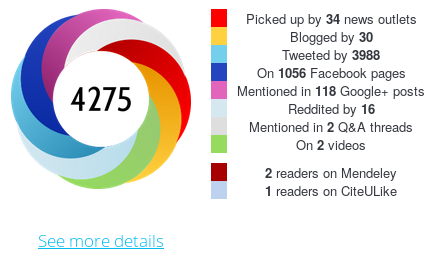
\includegraphics[width=0.7\linewidth]{imagenes/altmetrics_donough}
	\caption{Donut de Altmetric}
	\label{fig:altmetricsdonough}
\end{figure}


\subsection{Limitaciones}
Estas medidas ayudar dar una idea la importancia de un documento o de la productividad de un autor, pero no deben de ser tomadas como únicos criterios ya que presentan sus limitaciones.

Respecto a las medidas basadas en número de citas son muy dependientes de las fuentes de las que tomen datos así como su cobertura, por otro lado que un articulo sea muy citado no quiere decir que este sea muy influyente, se puede citar un trabajo para criticarlo. También hay que tener en cuenta las <<auto citas>> citas de un autor a otros trabajos suyos que pueden distorsionar estas medidas \cite{BibliometricWhitePaper}.

No se puede comparar categóricamente dos trabajos o autores de cualquier disciplina usándolas, ya que en distintos campos se cita de manera distinta. 

En las medidas que dependan de citaciones (prácticamente todas) hay que considerar un factor temporal, para que un trabajo adquiera relevancia es necesario cierto tiempo, por ello se recomienda dejar fuera las publicaciones recientes (de los últimos tres años)\cite{BibliometricWhitePaper}.
% Interesante hacer un apartado de plataformas bibliográficas ???


\section{Combinando ambas disciplinas}

En los últimos años han surgido diversos trabajos que proponen combinar ambas disciplinas, utilizar la bibliometría para mejorar la recuperación de información. Esto no se puede aplicar de manera genérica y directa a cualquier sistema de \acrshort{RI} ya que la bibliometría esta muy centrada en el mundo de la académico y de la investigación, sin embargo con algunas adaptaciones las ideas de la bibliometría se encuentran muy presentes en los sistemas de \acrshort{RI}, por ejemplo el algoritmo PageRank hace una analogía entre páginas web con artículos científicos así como hiperenlaces con citas en los mismos \cite{PageRankPaper}. 

\subsection{Sistemas de \acrshort{RI} actuales con medidas bibliométricas}
\label{subsec:sistemasRI}
Donde resulta obvio que esta combinación puede ser beneficiosa es los sistemas \acrshort{RI} especializados en literatura académica siendo los más importantes:

\begin{itemize}
	\item \href{https://scholar.google.es/}{Google Scholar}: buscador gratuito especializado en literatura científica, contiene algunas medidas bibliométricas con el número de citas o el índice-h de un autor. Sin embargo ha sido muy criticado por intentar incluir el mayor número de artículos posibles sin importar la calidad de los mismos \cite{googleScholarJunk} o dar demasiada importancia al número de citas lo que hace que sea complicado descubrir nuevos trabajos que no son muy conocidos \cite{Beel09}.
	
	\item \href{http://wos.fecyt.es/}{\acrfull{WoS}}: Sistema de RI por subscripción más utilizado, habitualmente las instituciones académicas lo tienen contratado, como es el caso de la \acrlong{UGR} a través de la \acrfull{FECYT}. Agrupa múltiples bases de datos de diversas índoles llegando a tener más de 100 millones de documentos \cite{WoS_Facts}. Fue uno de los primeros sistemas en aparecer y actualmente pertenece a Clarivate Analytics. A diferencia de Google Scholar los contenidos son revisados por expertos antes de ser incluidos \cite{WoS_Facts}. 
	
	\item \href{https://www.scopus.com/}{Scopus}: Similar a \acrshort{WoS}, en este caso pertenece a la editorial Elsevier. También se puede usar desde la \acrshort{UGR} gracias a la \acrshort{FECYT}. Este sistema es más reciente, cuenta con unos 70 millones de documentos \cite{scopus} y también tiene un proceso de revisión de contenido. Dispone de algunas otras medidas de bibliometría además del número de citas o índice-h, como los otros sistemas descritos, cuenta con las medidas \textit{CiteScore}, \textit{SCImago Journal Rank} y \textit{SNIP} (ver \ref{numero_citas} para más información). 
\end{itemize}

\subsection{Trabajos relacionados}
\label{subsc:trabajosRelacionados}
Desde un punto de vista académico resultan especialmente interesantes los trabajos de los talleres \acrfull{BIR}. Estos congresos se celebran anualmente desde 2014 y tienen como objetivo "\textit{hacer consciente a la comunidad de \acrshort{RI} de sus posibles vínculos con la bibliometría}" \cite{DBLP:conf/ecir/X14}. Voy a destacar algunos de ellos a continuación.

% Re ordenar resultados usando alguna medida, uso de altmetrics
Ante el creciente volumen de trabajos científicos se hace complicado para investigador mantenerse al día en su propio campo porque resulta imposible leer todos los trabajos, por ello se suele utilizar algún \gls{recomenderSystem} \glsrefentry{recomenderSystem}. Pero los sistemas existentes no contemplan bien el uso de medidas bibliométricas para distinguir los trabajos relevantes, por ello en \cite{DBLP:conf/ecir/SiebertDF17} se propone reordenar la salida del sistema de recomendación \href{mr-dlib.org}{\acrshort{Mr.DLib}} utilizando como criterio varias medidas derivadas del número de lectores de un artículo, un tipo de \textit{altmetric} (ver \ref{altmetrics}). Las conclusiones de este trabajo demuestran que se encuentra una mejora utilizando las medidas de cienciometría solas o en combinación con el ordenamiento normal basado en texto que usando solo el ordenamiento del sistema \acrshort{RI}, siendo la métrica que mejor resultado obtuvo el número absoluto de lecturas sin normalización. Esta mejora no es muy significativa como cabría esperar, los autores achacan esto a la falta de cobertura de datos bibliométricos en la colección.

% Modelo más clásico, priores con medidas biblio
Otro enfoque interesante es el de \cite{DBLP:conf/ecir/ZhaoH14}, donde se propone utilizar medidas bibliométricas como variables independientes de consulta o \textit{static features}, ver el modelo probabilístico \ref{modelProb}. Estás características se conocen como priores en el modelo probabilístico de lenguaje utilizado y modifican la probabilidad de que un documento sea relevante para una consulta dada, multiplicando dicha probabilidad por un factor. Para realizar su estudio han utilizado la colección bibliográfica de prueba iSearch, que desgraciadamente parece no estar disponible ya. De esta colección seleccionaron el subconjunto de artículos con al menos alguna cita dentro de la colección (para poder llevar acabo un análisis de co-citación). 

Como \textit{static features} específicas han seleccionado la proporción de citas dentro del subconjunto de documentos entre el número total de estas, el \textit{PageRank} calculado en el subconjunto y el clustering de co-citación \footnote{Creando un grafo no dirigido con peso de citas donde los nodos son documentos y las aristas citas, sobre el que se aplica un algoritmo de clustering y se calculan los priores del cluster mediante validación cruzada de 5 iteraciones.}, siendo todas las variantes también suavizadas con una versión logarítmica. Aunque el concepto es interesante y el método exhaustivo los resultados obtenidos no son significativos, se achaca esto al bajo tamaño de la colección de prueba, con 863 documentos.

% Otro modelo clásico, tf*idf sobre trabajos en lugar de términos usando co-citación como métrica
Siguiendo un modelo vectorial pero aplicando una variación del conocido esquema de pesos \textit{tf*idf} se encuentra \cite{DBLP:conf/ecir/White16}. En el esquema de ponderación para los términos original \textit{tf} representa la frecuencia de un término en el documento e \textit{idf} el número de documentos donde aparece el término a la inversa. Con ello se consigue dar mayor importancia a los términos que aparezcan menor número de veces ya que serán más discriminantes e importantes para una búsqueda.

El modelo propuesto en este paper apuesta por buscar documentos en función de otros, es decir los términos de consulta son otros documentos de la colección, los cuales se conocen como semillas. Para la ponderación de peso en cada documento ahora \textit{tf} es el número de documentos co-citados con el documento semilla e \textit{idf} la inversa del número total de citas entre documentos de la colección. Por último cita algunos ejemplos sobre colecciones de prueba y discute el modelo planteado sin llegar a evaluarlo realmente. De este, se dice que sería especialmente útil para usuarios con conocimiento previo del dominio, por ejemplo para llevar acabo una investigación bibliográfica sobre algún autor.

Basado parcialmente en el trabajo previo, el siguiente artículo \cite{DBLP:conf/ecir/SarolLS18} propone la creación de un \gls{framework} \glsrefentry{framework} para llevar a cabo una investigación bibliográfica siguiendo un enfoque híbrido combinando información textual y de citación. A partir de la selección de algunos documentos semilla, el sistema crea el espacio de citaciones \footnote{Documentos citados por las semillas, aquellos que las citan a ellas y documentos con relación de co-citación con estas.}, sobre el cual se filtra poniendo condiciones, el resultado de este filtrado se refina buscando términos y frases comunes con las semillas en el resumen de los documentos. 

Utilizan su sistema para comparar con diversos trabajos de revisión bibliográfica realizados manualmente con el objetivo de lograr obtener el mismo conjunto final de documentos relevantes revisando menos trabajos con lo que se ahorraría un tiempo significativo. Sus resultados resultan prometedores, usando todas las combinaciones de 3 documentos semilla entre los seleccionados finalmente por cada revisión logran recuperar todos los documentos finales disponibles en Scopus (plataforma en la que realizan el estudio) reduciendo el número de documentos totales recuperados para esa revisión en hasta el 80 \% dependiendo de la revisión concreta.




